\documentclass[10pt,twocolumn]{article}
\usepackage[utf8]{inputenc}
\usepackage[english]{babel}
\usepackage{amsmath, amssymb, amsthm}
\usepackage{graphicx, subfigure, epsfig}
\usepackage{geometry}
\usepackage{color, xcolor}
\usepackage{hyperref}
\usepackage{parskip}
\usepackage{tikz}
\usetikzlibrary{shapes,arrows}
\tikzstyle{block} = [rectangle, draw, text width=7.5em, text centered, rounded corners, node distance=4cm, minimum height=4em]
\tikzstyle{line} = [draw, -latex']
\usepackage{appendix}
\usepackage{caption}

\hypersetup{
	colorlinks,
	linkcolor={red!50!black},
	citecolor={blue!50!black},
	urlcolor={blue!80!black}
}

\newtheorem{eg}{Example}[section]

\begin{document}
	\title{Planeador de Excursiones}
	\author{
		Amanda Cordero Lezcano\\
		Christopher Guerra Herrero\\
		Alfredo Nuño Oquendo\\Facultad de Matemática y Computación, Universidad de La Habana
	}
	\date{Septiembre, 2024}
	
	\twocolumn[
	\begin{@twocolumnfalse}
		\maketitle
		\begin{abstract}
			Esta investigación presenta una simulación de un grupo de personas en una excursión, donde se recolectan características de los excursionistas mediante encuestas. Posteriormente, utilizando un algoritmo A*, se planifica una ruta que maximice la satisfacción de los participantes. De esta, se elabora un pequeño anuncio por medio de un modelo de lenguaje. Finalmente, se simula la excursión con un modelo basado en agentes BDI y un controlador difuso para ajustar los tiempos de espera y velocidad de los excursionistas en diferentes puntos del recorrido. Se destacan los puntos críticos que podrían utilizarse para mejorar futuras excursiones reales.
		\end{abstract}
		\vspace{1cm}
	\end{@twocolumnfalse}
	]
	\section{Introducción}
	\subsection{Breve descripción del proyecto}
	El objetivo de esta investigación es simular una excursión con un grupo de excursionistas basándose en sus preferencias individuales, las características del terreno y las rutas disponibles. Para ello, se recolecta información de los excursionistas a través de encuestas y se utiliza un algoritmo A* para maximizar su satisfacción durante el recorrido. Se elabora un anuncio usando el modelo de lenguaje Phind-34B. Se simula mediante agentes BDI, usando un controlador difuso para computar la velocidad y el tiempo de espera de los campistas.
	
	\subsection{Objetivos}
	Los principales objetivos de esta investigación son:
	\begin{itemize}
		\item Planificar rutas óptimas que maximicen la satisfacción de los excursionistas.
		\item Elaborar un anuncio llamativo para los excursionistas.
		\item Detectar puntos críticos en el recorrido que puedan mejorar la experiencia en excursiones reales.
		\item Crear una plataforma amigable para un potencial guía de la excursión.
	\end{itemize}
	
	\section{Fundamento Matemático}
	En esta sección se presentan los fundamentos matemáticos de las técnicas utilizadas para implementar la simulación: el algoritmo A*, el modelo de agentes BDI y el control difuso.
	
	\subsection{Algoritmo A*}
	El algoritmo A* es un método de búsqueda de caminos óptimos en un grafo ponderado. Se utiliza para encontrar la ruta más corta desde un punto de inicio hasta un destino, minimizando una función de evaluación \(f(n)\) que combina el costo actual y una estimación heurística:
	\[
	f(n) = g(n) + h(n)
	\]
	
	Donde:
	\begin{itemize}
		\item \(g(n)\) es el costo acumulado desde el inicio hasta el nodo \(n\),
		\item \(h(n)\) es la heurística que estima el costo restante desde \(n\) hasta el destino.
	\end{itemize}
	
	La heurística debe ser admisible, es decir, nunca debe sobrestimar el costo real para asegurar la optimalidad del algoritmo:
	\[
	h(n) \leq h^*(n) \quad \forall n
	\]
	
	El algoritmo A* es completitud y óptimo si la heurística es admisible.
	
	\subsection{Modelo de Agentes BDI}
	El modelo BDI (Belief-Desire-Intention) se basa en la lógica modal para representar el comportamiento racional de los agentes. Los agentes tienen:
	\begin{itemize}
		\item **Creencias** (\(B\)): Representan lo que el agente sabe o cree acerca del mundo.
		\item **Deseos** (\(D\)): Los objetivos que el agente intenta alcanzar.
		\item **Intenciones** (\(I\)): Los planes o acciones que el agente ha decidido ejecutar para lograr sus deseos.
	\end{itemize}
	
	Matemáticamente, el comportamiento de los agentes se puede describir usando una estructura modal \( \langle B, D, I \rangle \), donde cada componente se actualiza según las reglas del sistema. La lógica BDI sigue el principio de que las intenciones deben ser consistentes con las creencias y deseos actuales.
	
	\subsection{Controlador Difuso}
	
	En general, los controladores difusos son sistemas expertos especiales. Cada uno emplea una base de conocimientos, expresada en términos de reglas de inferencia difusa relevantes, y un motor de inferencia adecuado para resolver un problema de control determinado. Los controladores difusos varían sustancialmente según la naturaleza de los problemas de control que se supone deben resolver. Los problemas de control van desde tareas complejas, típicas en robótica, que requieren una multitud de acciones coordinadas, hasta objetivos simples, como mantener un estado prescrito de una sola variable.\cite{Fuzzy}
	
	Un controlador difuso general consiste en cuatro módulos: una base de reglas difusas, un motor de inferencia difusa, y módulos de fuzzificación/defuzzificación. Las interconexiones entre estos módulos y el proceso controlado se muestran en la Figura \ref{fig:diagram}.
	

	\begin{figure*}[h]
		\centering
		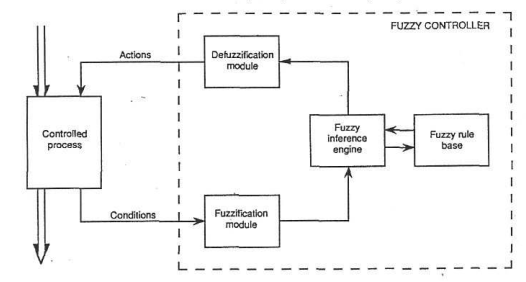
\includegraphics[width=\linewidth]{diagram}
		\caption{Imagen extraída de \cite{Fuzzy}. Esquema general de un controlador difuso}
		\label{fig:diagram}
	\end{figure*}
	
	
	
	%Un controlador difuso opera repitiendo un ciclo de los siguientes cuatro pasos. Primero, se toman mediciones de todas las variables que representan las condiciones relevantes del proceso controlado. Luego, estas mediciones se convierten en conjuntos difusos apropiados para expresar incertidumbres en las mediciones. Este paso se llama fuzzificación. Las mediciones fuzzificadas luego se utilizan por el motor de inferencia para evaluar las reglas de control almacenadas en la base de reglas difusas. El resultado de esta evaluación es un conjunto difuso (o varios conjuntos difusos) definidos en el universo de posibles acciones. Este conjunto difuso se convierte, en el paso final del ciclo, en un único valor (o un vector de valores) que, en cierto sentido, es el mejor representante del conjunto difuso (o conjuntos difusos). Esta conversión se llama defuzzificación. Los valores defuzzificados representan las acciones que toma el controlador difuso en ciclos individuales de control.\cite{Fuzzy}%
	 
	\section{Detalles de Implementación}
	
	\subsection{Pasos seguidos para la implementación}
	Se desarrolló un sitio web en Django para interactuar con el guía de la excursión. En la misma se encuentra una encuesta para los excursionistas, con la cual se obtendrán datos sobre sus preferencias. Posteriormente, el guía puede introducir en la plataforma el mapa de la región de interés. Usamos A* para planificar una ruta óptima en función de las preferencias y características del terreno. Luego se muestra en la web un anuncio elaborado por el modelo de lenguaje Phind-34B, a partir de las características del camino seleccionado.\\
	Para la simulación se modelan los excursionistas con agentes BDI. Aquí se diferencia el agente que representa al guía del resto de los excursionistas, debido a que entre los deseos del guía se encuentra también garantizar un recorrido seguro. Para los excursionistas se utiliza un controlador difuso; con las creencias de estos(características del mapa hasta el punto recorrido) y sus deseos(características recogidas en la encuesta) se aplican reglas como:
	
	$$
	 \mu_{\text{gusto\_historia\_bajo}} \implies \mu_{\text{tiempo\_espera\_corto}}
	$$
	Esta regla indica que si el gusto del usuario por la historia es bajo, entonces el tiempo de espera será corto.
	
	$$
	\mu_{\text{gusto\_historia\_medio}} \land \mu_{\text{indice\_historia\_bajo}}$$
	$$\implies \mu_{\text{tiempo\_espera\_corto}}$$
	
	
	Aquí se establece que si el gusto del usuario por la historia es medio y el índice de lugares históricos en el lugar es bajo, entonces el tiempo de espera será corto.
	
	$$
		\mu_{\text{gusto\_historia\_medio}}  \land $$
		 $$ \left( \mu_{\text{indice\_historia\_medio}}	
		 \lor \mu_{\text{indice\_historia\_alto}} \right)$$
		$$\implies \mu_{\text{tiempo\_espera\_medio}}$$

	Esta regla señala que si el gusto del usuario por la historia es medio y el índice de lugares históricos en el lugar es medio o alto, entonces el tiempo de espera será medio.
	
	
	
	\textbf{Descripción de Variables}
	\begin{itemize}
		\item \(\mu_{\text{gusto\_historia\_bajo}}\): Función de pertenencia que describe un bajo gusto del usuario por la historia.
		\item \(\mu_{\text{gusto\_historia\_medio}}\): Función de pertenencia que describe un gusto medio del usuario por la historia.
		\item \(\mu_{\text{indice\_historia\_bajo}}\): Función de pertenencia que describe un índice bajo de sitios históricos en el lugar.
		\item \(\mu{\text{indice\_historia\_medio}}\): Función de pertenencia que describe un índice medio de sitios históricos en el lugar.
		\item \(\mu_{\text{indice\_historia\_alto}}\): Función de pertenencia que describe un índice alto de sitios históricos en el lugar.
		\item \(\mu_{\text{tiempo\_espera\_corto}}\): Función de pertenencia que describe un tiempo de espera corto para el usuario.
		\item \(\mu_{\text{tiempo\_espera\_medio}}\): Función de pertenencia que describe un tiempo de espera medio para el usuario.
	\end{itemize}
	
	\section{Resultados y Experimentos}
	
	\subsection{Hallazgos de la simulación}
	El sistema logra planificar rutas que maximizan la satisfacción de los excursionistas. Los puntos con mayores índices de interés (fauna, flora, dificultad) resultan ser los más valorados.
	
	\subsection{Hipótesis extraídas de los resultados}
	Se plantea que ajustar las rutas en función de los puntos de mayor interés puede incrementar significativamente la satisfacción de los excursionistas. Además, mantener a los excursionistas juntos utilizando la supervisión del guía reduce la dispersión del grupo.
	
	\subsection{Experimentos realizados para validar las hipótesis}
	Se realizaron simulaciones con diferentes configuraciones de excursionistas y mapas para validar las hipótesis. En todos los casos, las rutas calculadas con A* maximizaron la satisfacción según las características de los puntos de interés y caminos.
	
	\section{Conclusiones}
	La simulación realizada permite planificar rutas óptimas para excursiones basadas en las preferencias individuales de los excursionistas y las características del terreno. La supervisión constante del guía ayuda a mantener la cohesión del grupo, y el modelo BDI con control difuso optimiza los tiempos de espera y velocidades en cada sección del recorrido.
	
	\begin{thebibliography}{9}
		
		\bibitem{Fuzzy} Klir, G. J., \& Yuan, B. (1995). \textit{Fuzzy Sets and Fuzzy Logic: Theory and Applications}. Prentice Hall. Información extraída de las páginas 330-332.
		
	\end{thebibliography}
	
	
\end{document}
